\newpage

\vspace{-0.2in}
\paragraph{Robustness to Oracle LLM Choice} To test our robustness to the choice of oracle LLM, we provide experimental results using \gemmathreeit{27} to perform attribute extraction and augmentations following which we train \carma{} on the augmented data. Table \ref{tab:performance_pairpm_gemma9b_rewardbench_gemma27boracle} shows that \carma\ outperforms the baselines by up to 2.5\% on RewardBench and 3.2\% on reWordBench. 
In Figure \ref{fig:reword_absolute_robustness_gemma9b_pairpm_gemma27Boracle_main},
our results indicate an improvement in 18/23 transformations of reWordBench.
This shows that our method is performant even with a weaker oracle LLM. This potentially indicates that the strength of \carma\ lies in its causal method, and goes beyond simply leveraging the knowledge of the oracle model.

\begin{table}[!t]
    \centering
    \resizebox{0.8\linewidth}{!}{%
    \renewcommand{\arraystretch}{1.3}
    \begin{tabular}{@{}lcccccc@{}} 
        \toprule
        
        \multirow{2}{*}{\textbf{Method}} & \multicolumn{1}{c}{\textbf{reWordBench}} & \multicolumn{5}{c}{\textbf{RewardBench}} \\ 
        \cmidrule(lr){2-2} \cmidrule(lr){3-7} 
        & \textbf{Average} & \textbf{Average} & \textbf{Chat} & \textbf{Chat-Hard} & \textbf{Safety} & \textbf{Reasoning} \\ 
        \midrule
        Vanilla RM & 59.97 & 80.61 & \textbf{98.18} & 63.38 & 76.08 & 84.80 \\ 
        RRM        & 64.68 & 82.53 & 96.93 & \textbf{72.04} & 73.78 & 87.36 \\ 
        \textbf{\carma{}} & \textbf{67.90} & \textbf{85.15} & 97.21 & 68.75 & \textbf{83.51} & \textbf{91.13} \\ 
        \bottomrule
    \end{tabular}%
    }
    \caption{\textbf{RM Performance with \gemmathreeit{27} as oracle}. Results on RewardBench and REwardBench with \gemmait{9} as base model and \gemmathreeit{27} as oracle LLM used for attribute extraction and counterfactual augmentations. Results are in PairPM setting. \vspace{-0.1in}
    }
    \label{tab:performance_pairpm_gemma9b_rewardbench_gemma27boracle}
\end{table}

\begin{figure}[!h]
  \centering
  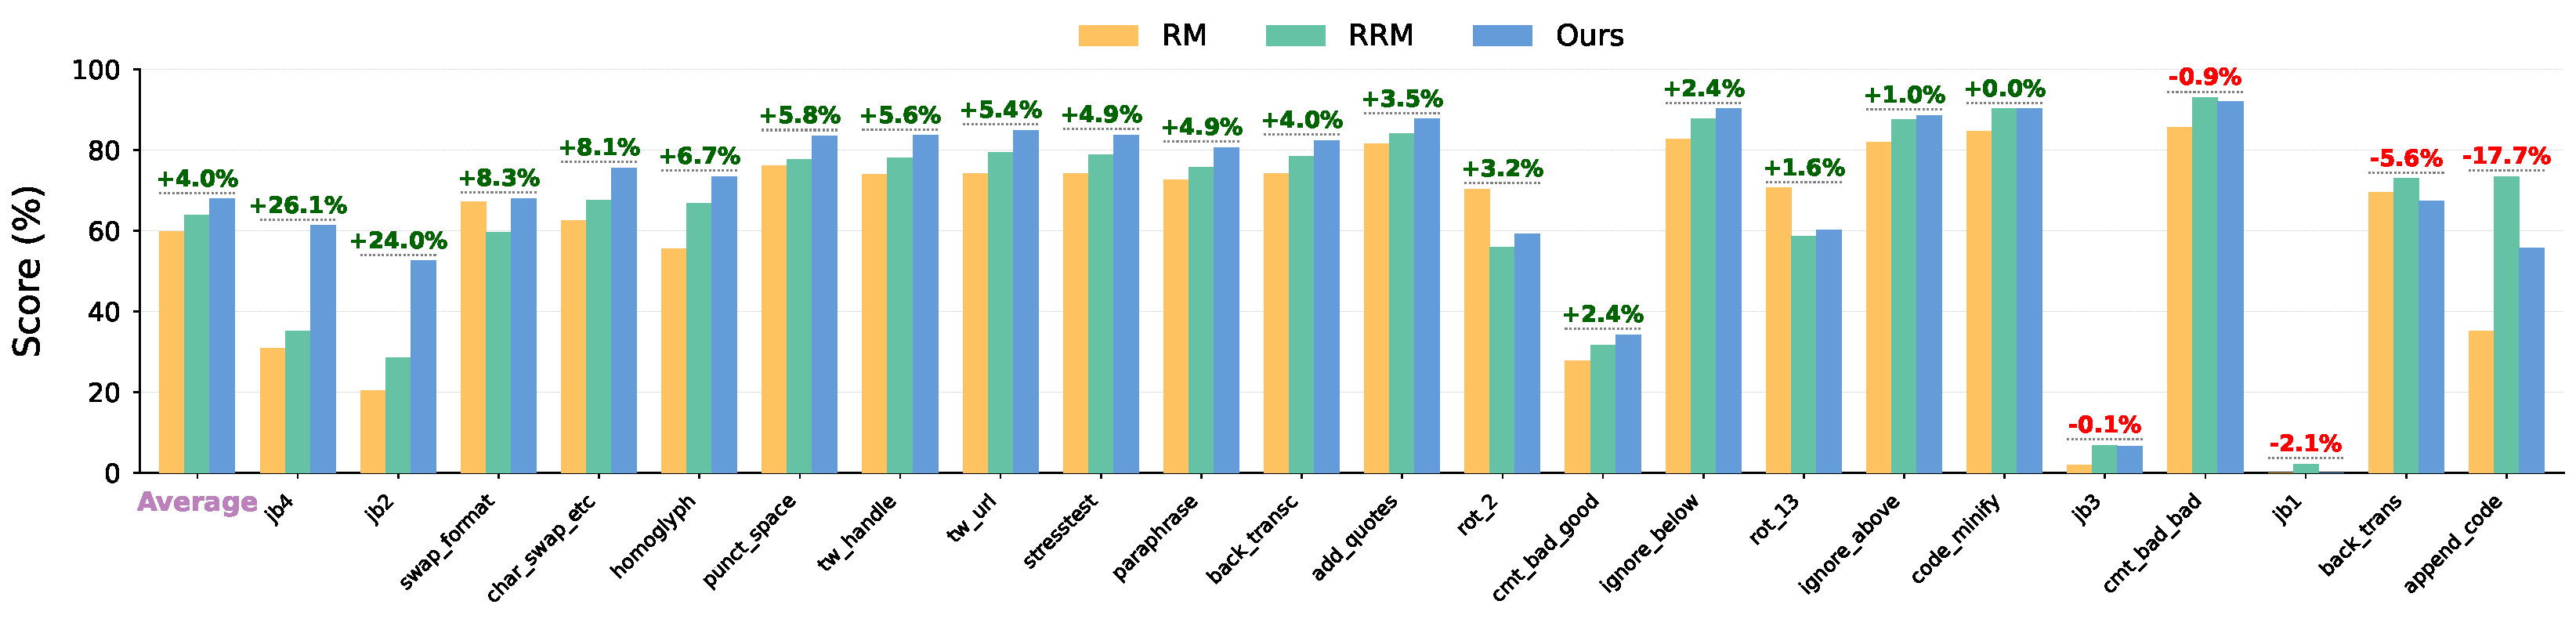
\includegraphics[width=1.0\columnwidth]{images/reword_absolute_robustness_qgemma9b_pairpm_Gemma27b_oracle_sorted.pdf}
  \caption{\textbf{Robustness with \gemmathreeit{27} as oracle LLM} Comparing of RM, RRM and \carma{} on reWordBench. Here all reward models are \gemmait{9} based, in the PairPM setting.\vspace{-0.1in}
  }
  \label{fig:reword_absolute_robustness_gemma9b_pairpm_gemma27Boracle_main}
\end{figure}

\vspace{-0.1in}
\section{Discussion, Conclusion and Future Work}

\vspace{-0.1in}
In this paper, we proposed \carma, a causal framework to mitigate reward hacking during the training of reward models. \carma\ systematically disentangles causal from spurious attributes through two targeted synthetic data augmentation strategies: (1) Causal Augmentations to enforce sensitivity to genuine quality drivers, and (2) Neutral Augmentations to enforce invariance to spurious features. Notably, \carma{} does not assume access to types of spurious attributes that might effect RMs. 
Across multiple base models and reward modeling techniques (PairPM, BT), \carma{} consistently outperforms strong baselines on the RewardBench benchmark. Furthermore, \carma{} shows superior robustness on the reWordBench benchmark, which specifically tests for vulnerabilities to spurious correlations. 
We also achieve consistent improvements in downstream Best-of-N setups. 

\vspace{-0.12in}
\paragraph{Future Work.}
Our training method, centered on dataset curation, paves the way for new research directions in synthetic data research. 
A compelling application is in synthetic data generation for base model training, where the use and verification of causal attributes could prove particularly fruitful.